	\documentclass[10pt,oneside]{CBFT_book}
	% Algunos paquetes
	\usepackage{amssymb}
	\usepackage{amsmath}
	\usepackage{graphicx}
	\usepackage{libertine}
% 	\usepackage[bold-style=TeX]{unicode-math}
	\usepackage{lipsum}

	\usepackage{natbib}
	\setcitestyle{square}

	\usepackage{polyglossia}
	\setdefaultlanguage{spanish}


	\usepackage{CBFT.estilo} % Cargo la hoja de estilo

	% Tipografías
	% \setromanfont[Mapping=tex-text]{Linux Libertine O}
	% \setsansfont[Mapping=tex-text]{DejaVu Sans}
	% \setmonofont[Mapping=tex-text]{DejaVu Sans Mono}

	%===================================================================
	%	DOCUMENTO PROPIAMENTE DICHO
	%===================================================================

\begin{document}

\chapter{Pequeñas oscilaciones}

Es un formalismo para analizar el movimiento que realiza un sistema cuando está sometido a
ligeras perturbaciones en la posición de equilibrio.
Esto desarrollará un método sistemático para tratar todo tipo de problemas con muchos grados
de libertad pero en forma aproximada.

\subsection{Idea para un grado de libertad}

Para un grado de liberada la idea es que 

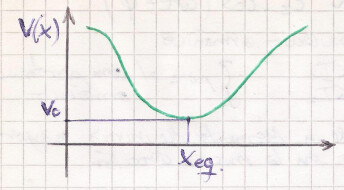
\includegraphics[scale=0.5]{images/fig_mc_oscil_1.jpg}

en un potencial $V(x)$ con un mínimo, es decir que cumple 
\[
	\dtot{V(x)}{x} = 0 ,\dtot[2]{V(x)}{x} > 0
\]
para algún $x_{eq}$, en la expresión de la energía
\be
	E = \frac 1 2 m \dot{x}^2 + V(x),
	\label{energia_1d}
\ee
se aproxima el potencial según\footnote{Nótese que esta es la expansión de Taylor en la cual el término lineal 
está justamente ausente porque la derivada primera en el punto es nula.}
\be
	V(x) \approx V_0 + \frac{1}{2} \left.\dtot[2]{V(x)}{x}\right|_{x_{eq}} (x-x_{eq})^2,
	\label{potencial_aproximado}
\ee
y si definimos $ k \equiv d^2V/dx^2|_{x_{eq}} $ se llega a 
\[
	E = \frac 1 2 m \dot{x}^2 + V_0 + \frac{1}{2} k (x-x_{eq})^2, 
\]
que derivada con respecto al tiempo resulta en 
\[
	m\ddot{x} + k (x-x_{eq}) = 0,
\]
la cual no es otra cosa que una ecuación de oscilador armónico, cuya solución general es
\[
	x(t) = A \cos (\omega t + \varphi ),
\]
donde $ \omega =  \sqrt{ k / m } $ y $ \varphi $ está asociada a la energía $E$. Ver Apéndice X para la resolución
de oscilador armónico.
\notamargen{Un apéndice más: oscilador armónico con término no homogéneo (usar 76R carpeta). Acá habría que llegar a despejar quién es
$\varphi$.}

El problema físico tiene dos constantes aunque la resolución presenta cuatro (dos complejos, con parte real e imaginaria).

Nótese que el desarrollo del potencial a orden dos equivale a una fuerza linealizada, merced a que $ m \ddot{x} = - dV/dx$.

\subsection{Varias variables}

En el caso de un potencial $V(\vb{x}_1, ...,\vb{x}_n)$ hay que hallar las raíces del mismo y luego desarrollar en torno a los puntos
de equilibrio. Se empieza desde 
\[
	\dpare{V}{\vb{x}}{x_{eq}} = 0,
\]
y habría que desarrollar 
\[
	V( \vb{x}_1, ...,\vb{x}_n ) = V( \vb{x}_1, ...,\vb{x}_n ) + 
	\frac 1 2 \sum_{i,j} \dparcru{V}{\vb{x}_i}{\vb{x}_j}(\vb{x}-\vb{x}_i)(\vb{x}-\vb{x}_j)
\]

No obstante, el problema se puede enfocar mejor en términos de las coordenadas generalizadas. Entonces, el potencial es
\[
	V(q_1,...,q_n) \approx V(q_1^0,...,q_n^0) + \sum_{i=1}^n \left. \dpar{V}{q_i} \right|_{q_i^0} (q_i - q_i^0)
		+ \frac{1}{2} \sum_{i,j=1}^n \left. \dparcru{V}{q_j}{q_i}\right|_{q_i^0}(q_i -q_i^0)(q_j -q_i^0)
\]
y la energía cinética,
\[
	T(q_1,...,q_n,\dot{q}_1,...,\dot{q}_n) \approx \frac{1}{2} \left( m(q_1^0,...,q_n^0) + \sum_{i=1}^n 
				\left. \dpar{m}{q_i} \right|_{q_i^0} (q_i - q_i^0) + ... \right) \sum_{i,j}^n \dot{q}_i\dot{q}_j
\]
[Esta expresión hay que revisarla y reubicarla!]

La energía cinética es 
\[
	T = \frac 1 2 \sum_{i,j} m_{ij}(q_1,...,q_n) \dot{q}_i \dot{q}_j
\]
donde $m_{ij}$ son los coeficientes de las coordenadas generalizadas y se desarrollarán en serie en torno al equilibrio (caracterizado
por un supraíndice $0$), es decir,
\[
	m_{ij} \approx m_{ij}( q_i^0, ..., q_n^0 ) + \sum_k \dpare{ m_{ij} }{ q_k }{q^0}( q_k - q_k^0 ).
\]

Estamos considerando que la energía cinética es $ T = T_2 $, pero cabría pensar que existe un $ T_0( q_1,...,q_n)$ y se lo 
sumaríamos en ese caso al potencial $V$. En el lagrangiano que consideraremos no está presente $T_1$; queremos un potencial
que no depende de las velocidades.

\begin{ejemplo}{Sobre el término $T_1$}

Para el caso de una masa fija, enhebrada en varilla que gira con velocidad angular $\omega$, el lagrangiano es
\[
	\Lag = \frac 1 2 m (\dot{r}^2 + r^2 \dot{\vp}^2),
\]
con energía
\[
	T = T_0 + T_2 = \frac{2}{2}mr^2\dot{\vp}^2 + \frac{2}{2}m\dot{r}^2
\]
donde $\dot{\vp} = \omega$ el último término no depende de la velocidad pero sí de la posición.
Es {\it como} un potencial que genera la fuerza ficticia.
\end{ejemplo}

\notamargen{Esta aproximación y formalismo sirve para un mínimo y un sistema que hace pequeños apartamientos
respecto de ese mínimo.}

Haciendo la aproximación consistente resulta 
\[
	\Lag = T - V = - \frac{1}{2} \sum_{i,j}^n \left. \dparcru{V}{q_j}{q_i}\right|_{q_i^0}(\eta_i)(\eta_j) +
		\frac{1}{2} \sum_{i,j}^n \left. m_{ij}\right|_{q_i^0} \dot{\eta}_i \dot{\eta}_j
\]
con $V_{ij} \equiv \partial^2 V / ( \partial q_i \partial q_j ) |_{q_i^0}, m_{ij} = m_{ij}|_{q_i^0}$, ambos simétricos, 
y donde se ha definido $\eta_i = q_i - q_i^0$, que es un apartamiento típico de la posición de equilibrio. 
Notemos que $\dot{q}_i = \dot{\eta}_i $. Nótese también que el término lineal en
la aproximación de $m_{ij}$ al verse multiplicado por el producto $\dot{q}_i\dot{q}_j$ es ya de orden cúbico por lo cual debe
descartarse para ser consistentes con las aproximaciones hechas en el potencial.

Con esta nomenclatura puede escribirse el {\it lagrangiano de pequeñas oscilaciones}
\[
	\Lag = \frac{1}{2} \sum_{i,j=1}^n m_{ij} \dot{\eta}_i \dot{\eta}_j - \frac{1}{2} \sum_{i,j=1}^n V_{ij} \eta_i \eta_j
\]
siendo ambas sumatorias formas bilineales cuadráticas reales y definidas positivas. Matricialmente,
\[
	\Lag = \frac{1}{2} \dot{\vb{\eta}}^t \mathbb{T} \dot{\vb{\eta}} - \frac{1}{2} \dot{\vb{\eta}}^t \mathbb{V} \dot{\vb{\eta}}
\]
y si ahora evaluamos las ecuaciones de Euler-Lagrange para este formalismo resulta que 
\[
	\frac{d}{dt}\left( \dpar{\Lag}{\dot{\eta}_k} \right) - \dpar{\Lag}{\eta_k} = 
		\frac{d}{dt} \left( \frac{1}{2} \sum_{i,j=1}^n m_{ij} \frac{d}{d\dot{\eta}_k}(\dot{\eta}_i \dot{\eta}_j) \right) - 
		\frac{1}{2} \sum_{i,j=1}^n V_{ij} \frac{d}{d\eta_k} (\eta_i \eta_j) = 0
\]
son $n$ ecuaciones diferenciales de Euler, 
\[
	\sum_{j=1}^n m_{kj} \ddot{\eta}_j + V_{kj} \eta_j = 0 \qquad k=(1,...,n).
\]

Esto es un oscilador armónico para cada partícula. Se puede pensar en todas las partículas unidas por resortes acoplados.

Se propone como solución 
\[
	\eta_j(t)  = A_j e^{i\omega t}
\]
de frecuencia $\omega$, idéntica para todas las partículas, tomando al final del proceso $\Re\{A_j e^{i\omega t}\}$ como 
solución física. Esta elección lleva a
\[
	\sum_{j=1}^n ( - \omega^2 m_{kj} + V_{kj} ) A_j = 0
\]
que equivale a
\[
	(\mathbb{V} -\omega^2\mathbb{T})\vb{A} = 0
\]
que no es otra cosa que un problema de autovalores y autovectores generalizado. Necesito
\[
	\left| \mathbb{V} -\omega^2\mathbb{T} \right| = 0
\]
lo cual me hará buscar un polinomio característico $P^n[\omega^2]$ de orden $n$ en $\omega^2$.
Así se trendrán $n$ valores para $\omega^2$ con $\omega^2_s \in \mathbb{R}$ y $\omega^2_s \geq 0$, que serán las
autofrecuencias o frecuencias propias $\omega^2_1, ...,\omega^2_n$. 

Para cada $\omega$ se tiene una solución
\[
	\eta_j^s = A_j^s e^{i\omega_s t}	 \qquad s=1,...,N
\]
pero el movimiento general será una combinación de todas las frecuencias,
\[
	\eta_j(t) = \sum_{s=1}^N c_s A_j^s e^{i\omega_s t}.
\]

En general, dado un $V=V(q_i)$ puede ser más fácil obtener explícitamente la serie de Taylor con 
$\partial^2 V/ \partial q_i \partial q_j |_{q_i^0}$ o bien cambiar variable $\eta = q_i - q_i^0$ y quedarse
con los términos cuadráticos en $\eta_i \eta_j$. Para la energía cinética $T=T(q,\dot{q})$ puede ser más
fácil evaluar $m_{ij}(q_i)|_{q_i^0}$ y quedarnos con los términos cuadráticos en $\dot{\eta}_i \dot{\eta}_j$.

Veamos la solución para una frecuencia dada,
\[
	\sum_j ( V_{kj} - \omega_s^2 m_{kj} ) A_j^s = 0
\]
y como usamos una raíz $\omega_s$ se tendrá una ecuación linealmente dependiente que tiraremos. Serán
ahora $N-1$ ecuaciones,
\[
	\sum_j ( V_{kj} - \omega_s^2 m_{kj} ) \frac{A_j^s}{A_1^s} = 0
\]
y definimos el cociente $a_j^s \equiv {A_j^s}/{A_1^s}$ al pasar dividiendo la amplitud del modo cuya frecuencia estamos
considerando. Entonces
\[
	\sum_j ( V_{kj} - \omega_s^2 m_{kj} ) a_j^s = - V_{k1} - \omega_s^2 m_{k1} \qquad k=1,...,N-1
\]
\notamargen{Acá sería bueno poner explícitamente hasta donde llega la sumatoria y explicitar qué $\omega$ se usa.}

Entonces como $N-1$ ecuaciones no homogéneas tienen solución real, entonces $a_j$ es un cociente real y todo los
$A_s^j$ tienen que tener la misma fase. [mmm?]

Veamos ahora que las frecuencias son reales. Para ello se multiplica por el complejo conjugado y se suma
\[
	\sum_k A_k^{s*} \sum_j V_{kj} A_j^s = \omega_s^2 \sum_k A_k^{s*} \sum_j m_{kj} A_j^s
\]
\[
	\sum_k A_k^{s} \sum_j V_{kj} A_j^{s*} = \omega_s^{2*} \sum_k A_k^{s} \sum_j m_{kj} A_j^{s*}
\]
y usando la simetría de $m_{kj}, V_{kj}$ se restan estas ecuaciones y se obtiene
\[
	0 = ( \omega^2_s - \omega^{2*}_s ) \sum_k \sum_j  A_k^{s*} m_{kj} A_j^{s}
\]
y como la doble sumatoria es no nula se sigue que las frecuencias son reales.
Incluso se puede despejar
\[
	\omega_s^2 = \frac{ \sum_k \sum_j  A_k^{s*} V_{kj} A_j^{s} }{ \sum_k \sum_j  A_k^{s*} m_{kj} A_j^{s} }
\]
Ambos, numerador y denominador son definidos positivos.
Si el numerador fuese negativo para alguna dirección, eso significa que en esa dirección será un máximo (sería una
especie de punto silla); pequeñas oscilaciones no valdrá en esa dirección.

Por otra parte, si se consideran dos frecuencias diferentes
\[
	0 = ( \omega^2_s - \omega^{2*}_p ) \sum_k \sum_j  A_k^{s*} m_{kj} A_j^{p}
\]
entonces lo que debe ser nulo es la doble sumatoria. Entonces, en la {\it métrica} dada por $m_{jk}$ $A_j$ y $A_k$
son perpendiculares.
Para determinar el $A_1$ impongo
\[
	{A^t}^{p*} M A^p = 1
\]
y los $A_j$ se {\it consideran} reales pués todos tienen la misma fase y son los modos normales.
Si construyo
\[
	A = \begin{pmatrix}
	A_1^1 & A_1^2 & ... \\
	A_2^1 &       &      \\
	...
	\end{pmatrix},
\]
donde cada columna de esta matriz es un autovector. Entonces
\[
	A^t V A = \begin{pmatrix}
	\omega_1^2 & 0 & ... \\
	0 &  \omega_2^2  &      \\
	...
	\end{pmatrix}.
\]

\begin{ejemplo}{\bf Lo de las matrices}

Si $ A^{p*} M A^s =0 $ con $ p \neq s $ entonces $M$ está definiendo una métrica pués si $ M = \mathbb{1} $ entonces
\[
	A^{p*} \mathbb{1} A^s = A^{p*} A^s = 0,
\]
lo cual significa que $A^{p*}$ y $ A^s$ son perpendiculares.
 
\end{ejemplo}


Vectorialmente es 
\[
	\vb{\eta}^s = \vb{A}_j^s e^{i\omega_s t} = \begin{pmatrix}
	                A_1 e^{i\omega_s t} \\
	                A_2 e^{i\omega_s t} \\
	                ... \\
	                A_N e^{i\omega_s t} \\
	               \end{pmatrix}
\]
para la frecuencia $\omega_s$, siendo cada uno un grado de libertad moviéndose con frecuencia $\omega_s$.

Luego, es
\[
	\vb{\eta}_{tot} = c_1 \vb{\eta}^1 + c_2 \vb{\eta}^2 + ... + c_N \vb{\eta}^N
\]
\[
	\vb{\eta}_{tot} = \begin{pmatrix}
				\eta_1 \\
				\eta_2 \\
				... \\
				\eta_n 
	                  \end{pmatrix}
	                 = \begin{pmatrix}
				c_1 A_1^1 e^{i\omega t} + c_2 A_1^2 e^{i\omega t} + ... + c_n A_1^n e^{i\omega t} \\
				c_1 A_2^1 e^{i\omega t} + c_2 A_2^2 e^{i\omega t} + ... + c_n A_2^n e^{i\omega t} \\
				... \\
				c_1 A_n^1 e^{i\omega t} + c_2 A_n^2 e^{i\omega t} + ... + c_n A_n^n e^{i\omega t}
	                  \end{pmatrix}
\]
entonces $\vb{A}^s$ es un modo normal de frecuencia $s$.
\[
	\vb{A}^s = \begin{pmatrix}
	            A_1^s \\
	            A_2^s \\
	            ... \\
	            A_n^s
	           \end{pmatrix}
	           e^{i\theta_0}
\]

La solución total ($j$ es el grado de libertad) se puede escribir 
\[
	\eta_j(t) = \sum_{s=1}^N c_s A_j^s e^{i\omega_s t}
\]
\[
	\vb{\eta}(t) = \sum_{s=1}^N c_s \vb{A}^s e^{i\omega_s t}
\]
y finalmente 
\[
	\vb{\eta}(t) = \Re \left\{ \sum_{s=1}^N c_s \vb{A}^s e^{i\omega_s t} \right\}
\]

Matricialmente,
\[
	\vb{A}^\dagger \mathbb{T} \vb{A} = 1
\]
siendo el $\dagger$ el traspuesto conjugado. Se pide que la norma (en la métrica dada por $\mathbb{T}$ de la unidad)
\[
	A^t \mathbb{T} A = \mathbb{1}
\]
lo cual significa que $A$ diagonaliza a $\mathbb{T}$, siendo 
\[
	A = \begin{pmatrix}
	     A_1^1 & A_1^2 & ... & A_1^n \\
	     A_2^1 & ... \\
	     A_n^1 & A_n^2 & ... & A_n^n 
	    \end{pmatrix}
\]
la matriz modal donde sus columnas son autovectores.

\[
	(\mathbb{V} - \omega^2 \mathbb{T})\vb{A} = 0
\]
interpolando a la matriz 
\[
	A^t \mathbb{V} A = \omega^2 A^t \mathbb{T} A= \omega^2 \mathbb{1}
\]
y sea ahora el siguiente cambio de coordenadas
\[
	\vb{\eta} = A \vb{\xi}
\]
tal que 
\[
	A^{n\times n} \xi^{n\times 1} \qquad \qquad  (A \vb{\xi} )^t = {\xi^t}^{1 \times n} {A^t}^{n \times n}
\]
y que se llaman coordenadas normales.

\[
	\Lag = \frac{1}{2} \dot{\vb{\eta}}^t \mathbb{T} \dot{\vb{\eta}} - \frac{1}{2} \dot{\vb{\eta}}^t \mathbb{V} \dot{\vb{\eta}}
\]
\[
	\Lag = \frac{1}{2} A^t\dot{\vb{\xi}}^t \mathbb{T} A \dot{\vb{\xi}} - \frac{1}{2} A^t\dot{\vb{\xi}}^t \mathbb{V} 
\dot{\vb{\xi}}
\]
\[
	\Lag = \frac{1}{2} \dot{\vb{\xi}}^t \mathbb{1} \dot{\vb{\xi}} - \frac{1}{2} \dot{\vb{\xi}}^t \omega^2 \mathbb{1} \dot{\vb{\xi}}
\]

\[
	\Lag = \frac{1}{2} \sum_i \dot{\vb{\xi}}_i^2 - \frac{1}{2} \sum_i \vb{\xi}_i^2 \omega^2_i 
\]
\[
	\frac{d}{dt}\left( \dpar{\Lag}{\dot{\xi}_i} \right)- \dpar{\Lag}{\xi_i} = \sum_i \ddot{\xi}_i + \omega^2_i \xi_i = 0 
\]
y son $N$ ecuaciones de Euler-Lagrange.
\[
	\sum_i ( -\omega^2 + \omega^2_i ) A_i = 0
\]
de modo que si $\omega^2 = \omega^2_i$ entonces
\[
	\xi_i = C_i e^{i\omega_i t}
\]

Digamos que en coordenadas normales
\[
	\xi_j = C_j e^{i \omega_j t}
\]
grados de libertad en $\xi$ (un grado de libertad es una $\omega$) y se desacoplan los grados de libertad
en lo que hace a $\omega_s$.
Por otro lado,
\[
	\eta_j = \sum_{s=1}^N c_s A_j^s e^{i \omega_j t}
\]
grados de libertad en $\eta$, un grado de libertad entonces es combinación lineal de todas las $\omega$.

Si $\omega=0$ es 
\[
	\xi_j = At + B 
\]
\[
	\eta_j = \sum_{s=1}^{N-1} c_s A_j^s e^{i \omega_j t} + A_j(Gt + D)
\]
siendo el último término asociado a la $\omega=0$.
Para volver atrás es 
\[
	A^{\dagger} \mathbb{T} A = \mathbb{1}
\]
y entonces 
\[
	A^{\dagger} \mathbb{T} \vb{\eta} = A^{\dagger} \mathbb{T} A \vb{\xi}  
\]
\[
	A^{\dagger} \mathbb{T} \vb{\eta} = \mathbb{1} \xi
\]
coordenadas normales en función de las de desplazamiento.

En conclusión podemos decir varias cosas,
\begin{itemize}
 \item Las frecuencias nulas están asociadas a momentos conservados.
 \item En coordenadas normales cada grado de libertad oscial con una frecuencia única (son $N$
	osciladores independientes)
 \item Las amplitudes cumplen
 \[ \vb{A}^s =
 \begin{pmatrix}
  a_1^s e^{i \phi_s} \\
  a_2^s e^{i \phi_s} \\
  ... \\
  a_n^s e^{i \phi_s}
 \end{pmatrix}
 \]
 donde tienen la misma fase los $A_j^s$ para toda frecuencia $\omega_s$
 \item Los modos normales pueden excitarse por separado (son ortogonales).
 \item Frecuencias iguales generarán modos normales que son físicamente los
 mismos. Son generados por la simetría del problema.
 \[
	\vb{A} = a_1(v_1) + a_2(v_2)
 \]
 si por ejemplo generan dos autovectores de esta forma.
\end{itemize}


% =================================================================================================
\section{Oscilaciones viscosas}
% =================================================================================================

\[
	\sum_j m_{ij} \ddot{\eta}_j + V_{ij}\eta_j + B_{ij}\dot{\eta}_j = 0
\]
no se puede convertir en osciladores independientes.
\[
	det\left\{ \mathbb{V} + \omega^2 \mathbb{T} + \omega \mathbb{B}\right\} = 0
\]


\begin{ejemplo}{\bf Problema 14 Método de Lagrange}

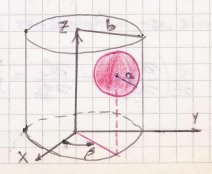
\includegraphics[scale=0.5]{images/fig_mc_lagrangebola_1.jpg}

El lagrangiano es
\[
	\Lag = \frac 1 2 m ( (b-a)^2 \dot{\beta}^2 + \dot{z}^2 ) + 
	\frac 1 2 I ( \dot{\vp}^2 + \dot{\theta}^2 + \dot{\psi}^2 + 2 \dot{\psi} \dot{\vp} \cos\theta ) 
	- m g z
\]
y como la velocidad $ \vb{v}_p $ es nula, se tiene 
\[
	\vb{v}_p = 0 = \vb{V}_{cm} + \vb{\Omega} \times a \hat{\vp}
\]
que lleva a
\[
	0 = (b-a)\dot{\beta}\hat{\beta} + \dot{z}\hat{z} +
	[\omega_\rho\hat{\rho} + \omega_\beta\hat{\beta} + \omega_z\hat{z} ]\times a\hat{\rho}
\]
\[
	0 = (b-a)\dot{\beta}\hat{\beta} + \dot{z}\hat{z} + a\omega_z\hat{\beta} - a\omega_\beta\hat{z} 
\]

La condición de rodadura es
\[
	\begin{cases}
	 (b-a)\dot{\beta} + a \omega_z = 0 \\
	 \dot{z} - a \omega_\beta = 0
	\end{cases}
\]
y como la velocidad en cartesianas es $ \vb{\Omega} = \Omega_x \hat{x} + \Omega_y \hat{y} + \Omega_z \hat{z} $,
la conversión a los ejes del problema es
\[
	\hat{\rho} = \cos \beta \hat{x} + \sin \beta \hat{y} \qquad 
	\hat{\beta} = -\sin \beta \hat{x} + \cos \beta \hat{y}
\]
o bien
\[
	\hat{x} = \cos \beta \hat{\rho} - \sin \beta \hat{\beta} \qquad 
	\hat{y} = \sin \beta \hat{\rho} + \cos \beta \hat{\beta}
\]
entonces
\[
	\vb{\Omega} = \omega_\rho \hat{\rho} + \omega_\beta \hat{\beta} + \omega_z \hat{z}
\]
donde 
\[
	\omega_\rho = \Omega_x \cos\beta + \Omega_y \sin\beta \qquad 
	\omega_\beta = \Omega_y \cos\beta + \Omega_x \sin\beta 
\]

Luego de algún álgebra
\[
	\omega_\rho = \dot{\psi} \sin\theta \sin(\vp-\beta) + \dot{\theta} \cos(\vp-\beta)
\]
\[
	\omega_\beta = -\dot{\psi} \sin\theta \cos(\vp-\beta) + \dot{\theta} \sin(\vp-\beta)
\]
\[
	\omega_z = \dot{\psi} \cos\theta + \dot{\vp}
\]

Pero como
\[
	(b-a) \beta + a \dot{\vp} + a \dot{\psi} \cos\theta = 0 ,
\]
\[
	\dot{z} -a \dot{\theta} \sin(\vp-\beta) + a\dot{\psi}\sin\theta\cos(\vp -\beta) = 0,
\]
conviene utilizar multiplicadores de Lagrange,
\[
	\dtot{}{t}\left( \dpar{\Lag}{\dot{q}_k} \right) - \dpar{\Lag}{q_k} = \sum_{\ell=1}^2 \lambda_\ell a_{\ell k}
\]
lo cual lleva a 
\[
	m(b-a)^2 \ddot{\beta} = \lambda_1 (b-a) \qquad \qquad 
	m \ddot{z} + m g = \lambda_2
\]
\[
	I \ddot{\vp} + I \dtot{}{t}( 2 \dot{\psi} \cos\theta ) = a \lambda_1
\]

Haciendo gradiente en los vínculos,
\[
	\lambda_1 ( [b-a] \delta\beta + a\delta\vp + a\cos\theta\delta\psi) = 0
\]
\[
	\lambda_2 (\delta z - a\sin(\vp-\theta)\delta\theta + a\sin\theta \cos(\vp-\beta)\delta\psi) = 0
\]
y entonces
\[
	I \ddot{\theta} +  I \dot{\psi} \dot{\vp} \sin\theta ) =
	- a \lambda_2 \vp \sin (\vp - \beta)
\]
\[
	I \ddot{\psi} +  I \dtot{}{t}( \dot{\psi} \cos\theta ) =
	\lambda_1 a \cos\theta + \lambda_2 \vp \sin \theta \cos(\vp - \theta)
\]

Tenemos siete ecuaciones con siete incógnitas. Una sugerencia para resolverlo alternativamente
es a través de las ecuaciones de Newton,
\[
	m\dot{\vb{V}_{cm}} = \vb{f} + \vb{N} \qquad \qquad 
	I \dot{\vb{\omega}} = \vb{t}
\]

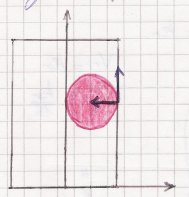
\includegraphics[scale=0.5]{images/fig_mc_lagrangebola_2.jpg}

\[
	\dtot{\omega}{t} = \left.\dtot{\omega}{t}\right| + \dot{\beta}\hat{\beta} \times \vb{\omega}
\]
lo cual nos debería conducir a algo de la forma
\[
	(I + ma^2)\ddot{\omega}\vp + \dot{\vp} I \omega_\vp = 0
\]
y sale que $\omega_\rho = \dot{\vp} \omega_\vp$ siendo $\dot{\vp}$ y $\dot{z}$ constantes.

\end{ejemplo}


\begin{ejemplo}{\bf Problema de la molécula diatómica}

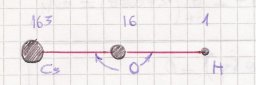
\includegraphics[scale=0.5]{images/fig_mc_molecula_1.jpg}

Acá hay que escribir el potencial con cuidado,
\[
	V = V_\alpha(\alpha) + V_{Cso}(r) + V_{OH}(r'),
\]
donde 
\[
	V_\alpha(\alpha) = \frac{k\ell^2}{2}(\pi - \alpha)^2
\]
y $\ell$ es un $r, r'$ de equilibrio.
\[
	V_{Cso}(r) = 4 \epsilon 
	\left[ \Frac{\sigma}{r}^{12} - \Frac{\sigma}{r}^6\right]
\]
\[
	V_{OH}(r') = \frac{V_{Cso}(r') }{15}
\]
y según se ve ya está separado el mismo.
Calculamos las derivadas del potencial,
\[
	V_{\alpha\alpha} = \dpar[2]{V}{\alpha} = k\ell^2 
\]
y de 
\[
	\dpar{V_{Cso}}{r}(r) = 0
\]
sale un $r_{eq}$ que cumple $r_{eq} = \sigma 2^{1/12}\equiv \ell$ y luego
\[
	\left. V_{Cso}{''}\right|_{eq} = 24 \epsilon 
	\left[ \frac{26}{r^2} \Frac{\sigma}{r}^{12} - \frac{7}{r^2} \Frac{\sigma}{r}^6\right] = k_r
\]
donde los términos con $\sigma$ equivalen a $4\ell^2$ y $2\ell^2$. Además,
\[
	V_{rr} = k_r \qquad V_{r'r'} = \frac{k_r}{15}
\]

Esto define
\[
	V = \begin{pmatrix}
	 V_{\alpha\alpha} & 0 & 0 & 0 \\
	 0 & V_{rr} & 0 & 0 \\
	 0 & 0 & V_{r'r'} & 0  \\
	 0 & 0 & 0 & ...
	 \end{pmatrix}
\]

En general tenemos más grados de libertad que tres. Ubicamos el centro de masa en
el Cesio por ser muy masivo. Entonces pierdo tres grados de libertad y me quedan
seis. Ignoro rotación, y otra cosa más [¿?]

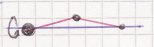
\includegraphics[scale=0.5]{images/fig_mc_molecula_3.jpg}

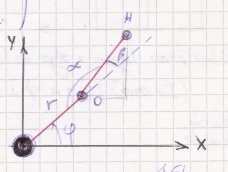
\includegraphics[scale=0.5]{images/fig_mc_molecula_2.jpg}

Restan cuatro grados de libertad $r, \vp, r', \beta$.
\[
	\dot{X}_0^2 = \dot{r}^2 + r^2 \dot{\vp}^2
\]
\[
	\vb{X}_0 = r \cos (\vp) \hat{x} + r \sin (\vp) \hat{y}
\]
\[
	\vb{X}_H = \vb{X}_0 + r' \cos (\vp + \beta) \hat{x} + r' \sin (\vp + \beta) \hat{y}
\]
y el cuadrado es
\[
	\dot{X}_H^2 = \dot{X}_0^2 + \dot{r'}^2 + {r'}^2 ( \dot{\vp} + \dot{\beta} )^2
\]
\begin{multline}
	2 \dot{r} \dot{r'} [ \cos \vp \cos (\beta + \vp) + \sin\vp \sin(\beta + \vp) ] + \\
	2 {r} {r'} [ \sin(\beta + \vp) \sin\vp (\dot{\beta} + \dot{\vp}) \dot{\vp} + \cos(\beta + \vp) \cos\vp \dot{\vp} (\dot{\beta} + \dot{\vp}) ] + \\
	2 \dot{r} {r'} [ \cos (\beta + \vp) \sin \vp - \cos \vp \sin (\beta + \vp)] (\dot{\beta} + \dot{\vp}) + \\
	2 {r} \dot{r'} [ \dot{\vp} \cos\vp \sin(\beta + \vp) - \dot{\vp} \sin\vp \cos (\beta + \vp)] 
\end{multline}
donde los últimos dos se {\it mueren} al aproximar.
Finalmente el lagrangiano de pequeñas oscilaciones resulta en
\[
	\Lag = \frac {17} 2 m ( \dot{r}^2 + r^2 \dot{\vp}^2 ) + 
	\frac m 2 ( \dot{r'}^2 + {r'}^2( \dot{\vp} + \dot{\beta} ) ) +
	\frac m 2 ( 2 \dot{r} \dot{r'} + 2 \ell^2 ( \dot{\beta} + \dot{\vp} ) \dot{\vp} ) - 
	\frac{k_r r^2}{2} - \frac{k_{r'} {r'}^2}{2} - \frac{k_\beta \beta^2}{2}
\]
en donde los $r^2$ y ${r'}^2$ son ambos $\ell^2$.
\end{ejemplo}


% \bibliographystyle{CBFT-apa-good}	% (uses file "apa-good.bst")
% \bibliography{CBFT.Referencias} % La base de datos bibliográfica

\end{document}
